\newcommand{\meanPerSampleScores}{
    \begin{table}[H]
        \centering
        \begin{tabular}{|P{3,2cm}||P{1,8cm} P{1,8cm} P{1,8cm} P{1,8cm} P{1,8cm}|}
            \hline
            Mean per-sample & \multicolumn{5}{c|}{\textbf{FPR}} \\
            tagging scores & $10^{-5}$ & $10^{-4}$ & $10^{-3}$ & $10^{-2}$ & $10^{-1}$ \\
            \hline
            \multicolumn{6}{|c|}{\textbf{Jaccard Similarity}} \\
            \hline
            ALOHA (M/B only) & - & - & - & - & - \\
            ALOHA & 0.674$\pm$0.004 & 0.716$\pm$0.013 & 0.787$\pm$0.014 & 0.864$\pm$0.003 & 0.793$\pm$0.002 \\
            Joint Embedding & \textBF{0.703$\pm$0.016} & \textBF{0.751$\pm$0.016} & 0.826$\pm$0.020 & \textBF{0.880$\pm$0.005} & 0.784$\pm$0.003 \\
            Proposed Model & 0.693$\pm$0.017 & 0.748$\pm$0.017 & \textBF{0.830$\pm$0.007} & 0.877$\pm$0.002 & \textBF{0.797$\pm$0.005} \\
            \hline
            \multicolumn{6}{|c|}{\textbf{Mean per-Sample Accuracy}} \\
            \hline
            ALOHA (M/B only) & - & - & - & - & - \\
            ALOHA & 0.633$\pm$0.002 & 0.658$\pm$0.014 & 0.716$\pm$0.031 & 0.791$\pm$0.002 & \textBF{0.699$\pm$0.003} \\
            Joint Embedding & 0.643$\pm$0.005 & 0.680$\pm$0.012 & 0.763$\pm$0.021 & 0.806$\pm$0.004 & 0.684$\pm$0.006 \\
            Proposed Model & \textBF{0.645$\pm$0.005} & \textBF{0.682$\pm$0.006} & \textBF{0.764$\pm$0.013} & \textBF{0.806$\pm$0.002} & 0.699$\pm$0.004 \\
            \hline
        \end{tabular}
        \caption[Tags prediction task mean per-sample scores]{Mean and standard deviation of mean per-sample tagging results (\textit{Jaccard simialrity} and \textit{mean per-sample accuracy}) for the different models. Results were aggregated over \textBF{3} training runs with different weight initializations and minibatch orderings. Best results are shown in \textbf{bold}.} \label{tab:meanPerSampleScores}
    \end{table}
}

\newcommand{\allMeanRocAlohaMB}{
    \begin{figure}[H]
        \vspace*{-0.5cm}
        \centering
        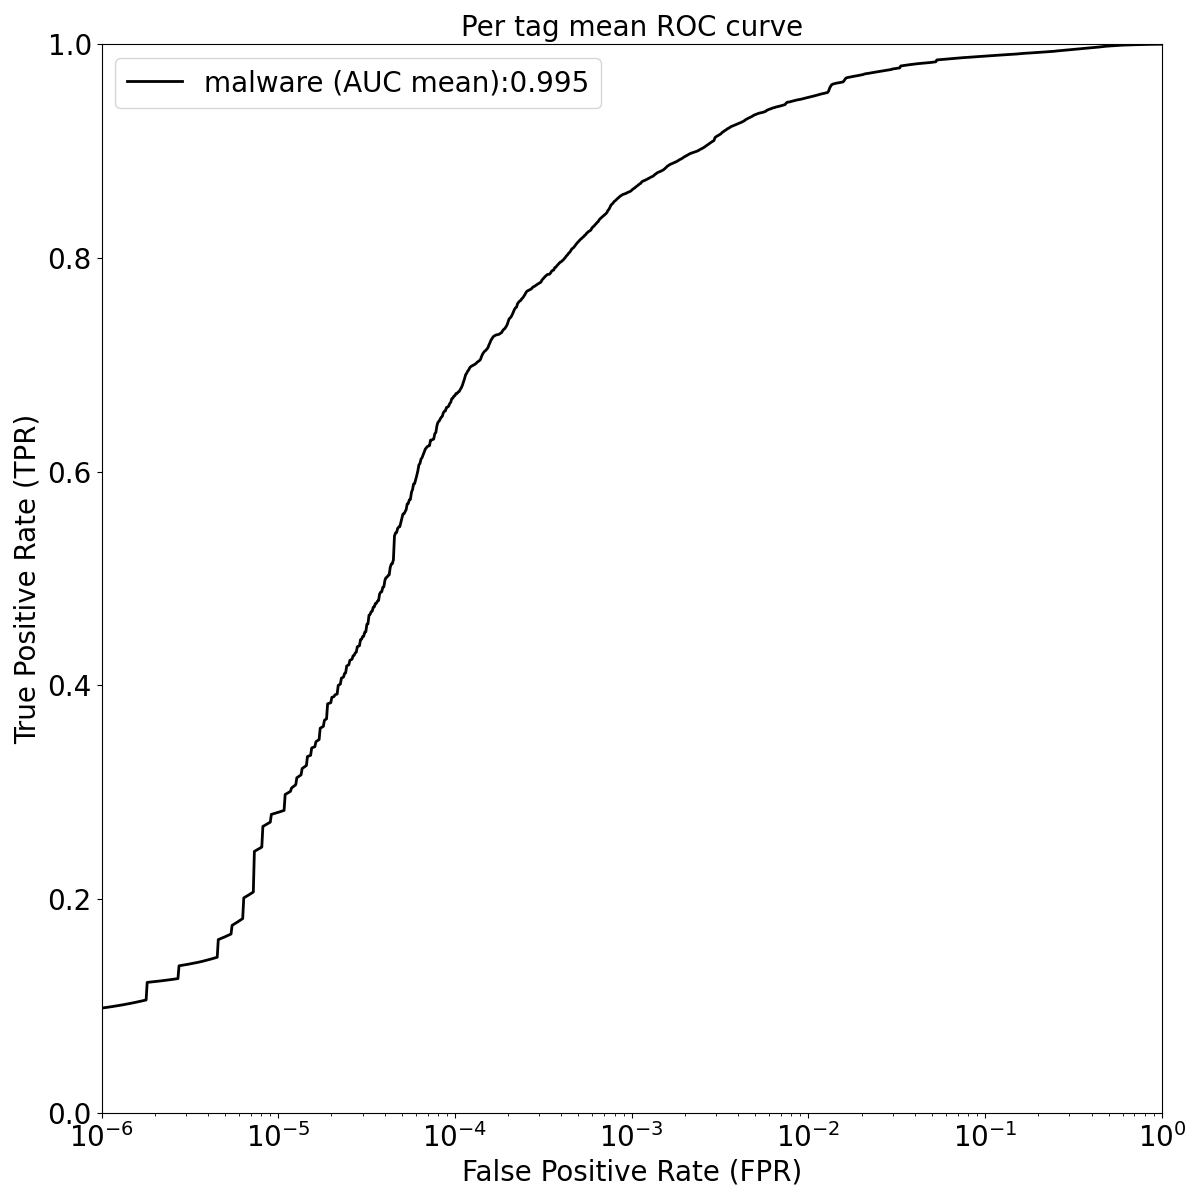
\includegraphics[width=0.6\textwidth]{./results/all_mean_roc_alohaMB.png}
        \vspace*{-0.2cm}
        \caption[Tags prediction task ALOHA (M/B only) mean ROC curve]{Mean ROC curve and AUC statistics of \textBF{ALOHA (M/B only)} model for the tags/labels. The line represents the \textit{mean} TPR at a given FPR. Statistics were computed over \textBF{3} training runs, each with random parameter initialization.}
        \label{fig:allMeanRocAloha}
    \end{figure}
}

\newcommand{\allMeanRocAloha}{
    \begin{figure}[H]
        \vspace*{-0.5cm}
        \centering
        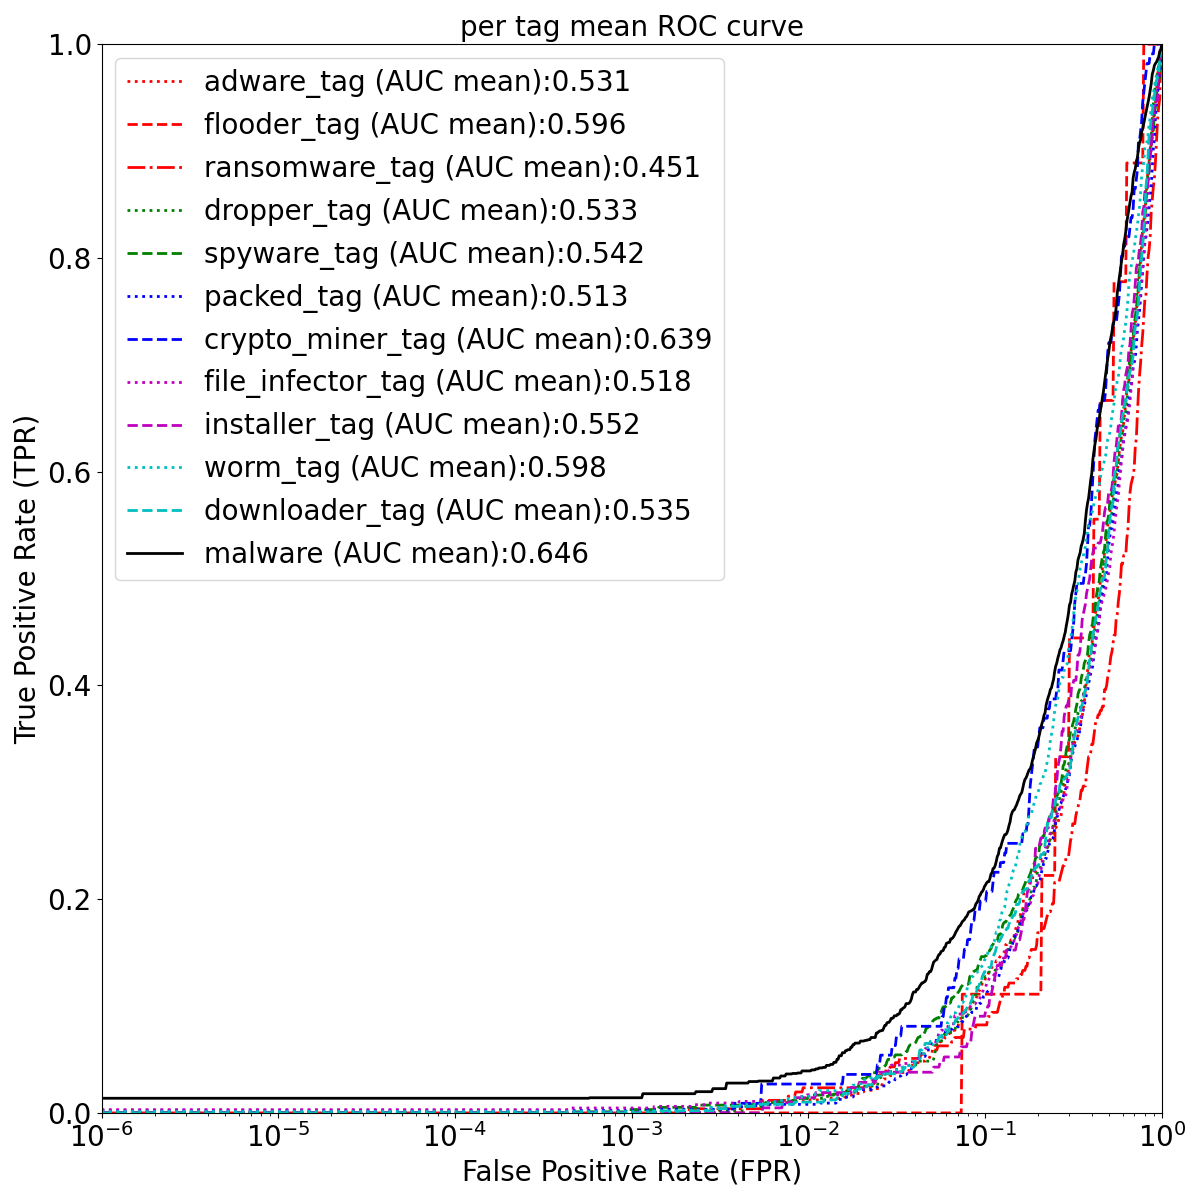
\includegraphics[width=0.6\textwidth]{./results/all_mean_roc_aloha.png}
        \vspace*{-0.2cm}
        \caption[Tags prediction task ALOHA mean ROC curve]{Mean ROC curve and AUC statistics of \textBF{ALOHA} model for the tags/labels. The line represents the \textit{mean} TPR at a given FPR. Statistics were computed over \textBF{3} training runs, each with random parameter initialization.}
        \label{fig:allMeanRocAloha}
    \end{figure}
}

\newcommand{\allMeanRocJointEmbedding}{
    \begin{figure}[H]
        \vspace*{-0.5cm}
        \centering
        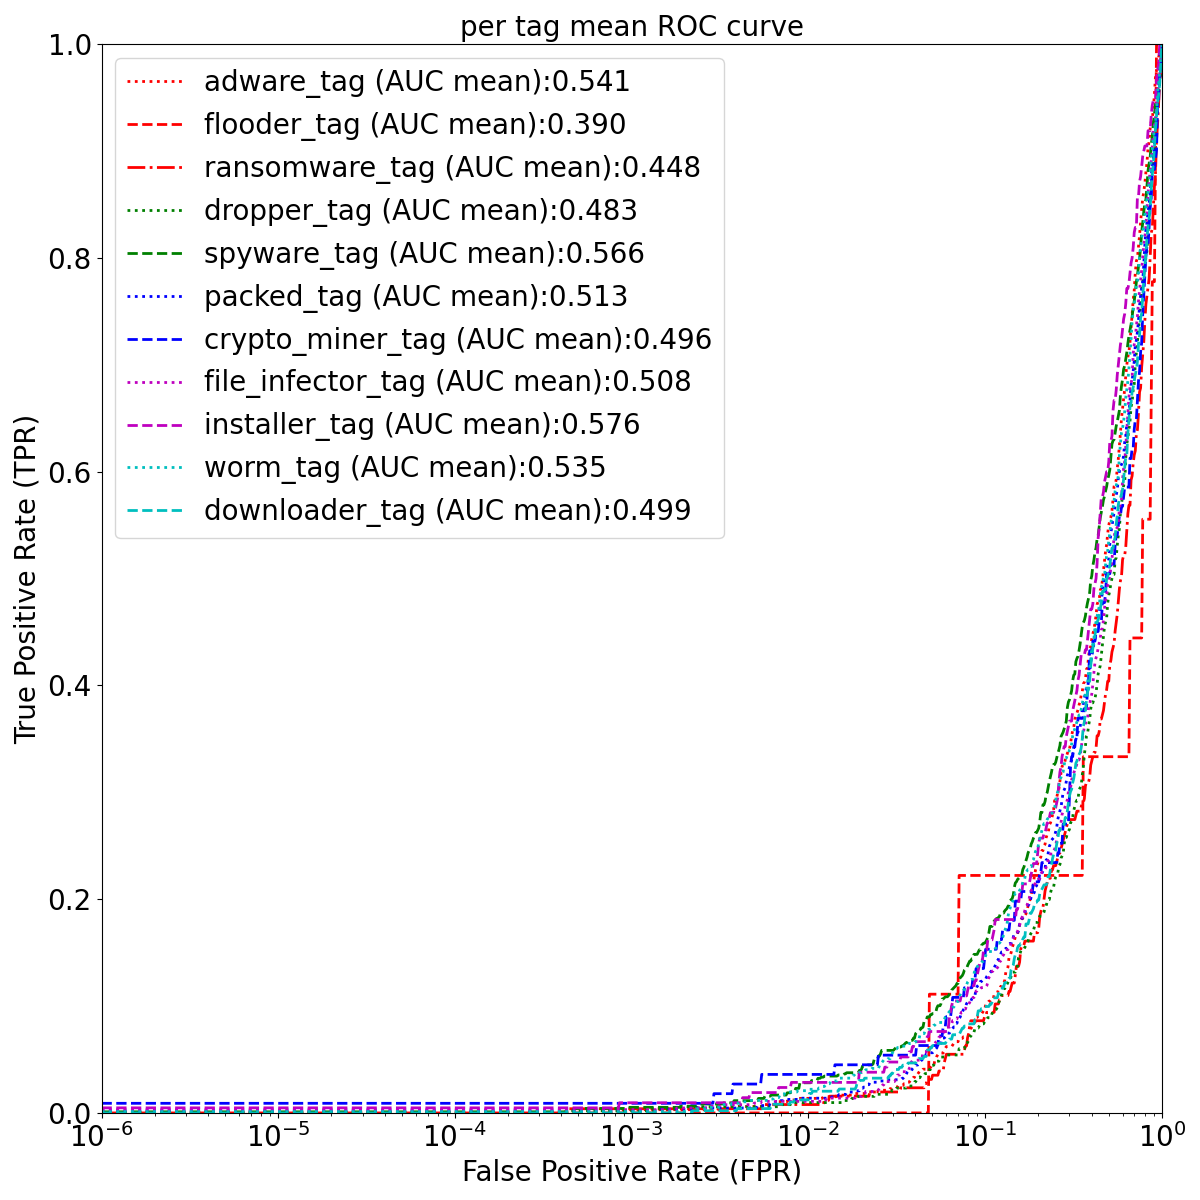
\includegraphics[width=0.6\textwidth]{./results/all_mean_roc_jointEmbedding.png}
        \vspace*{-0.2cm}
        \caption[Tags prediction task Joint Embedding mean ROC curve]{Mean ROC curve and AUC statistics of \textBF{Joint Embedding} model for all tags/labels. The line represents the \textit{mean} TPR at a given FPR. Statistics were computed over \textBF{3} training runs, each with random parameter initialization.}
        \label{fig:allMeanRocJointEmbedding}
    \end{figure}
}

\newcommand{\allMeanRocProposedModel}{
    \begin{figure}[H]
        \vspace*{-0.5cm}
        \centering
        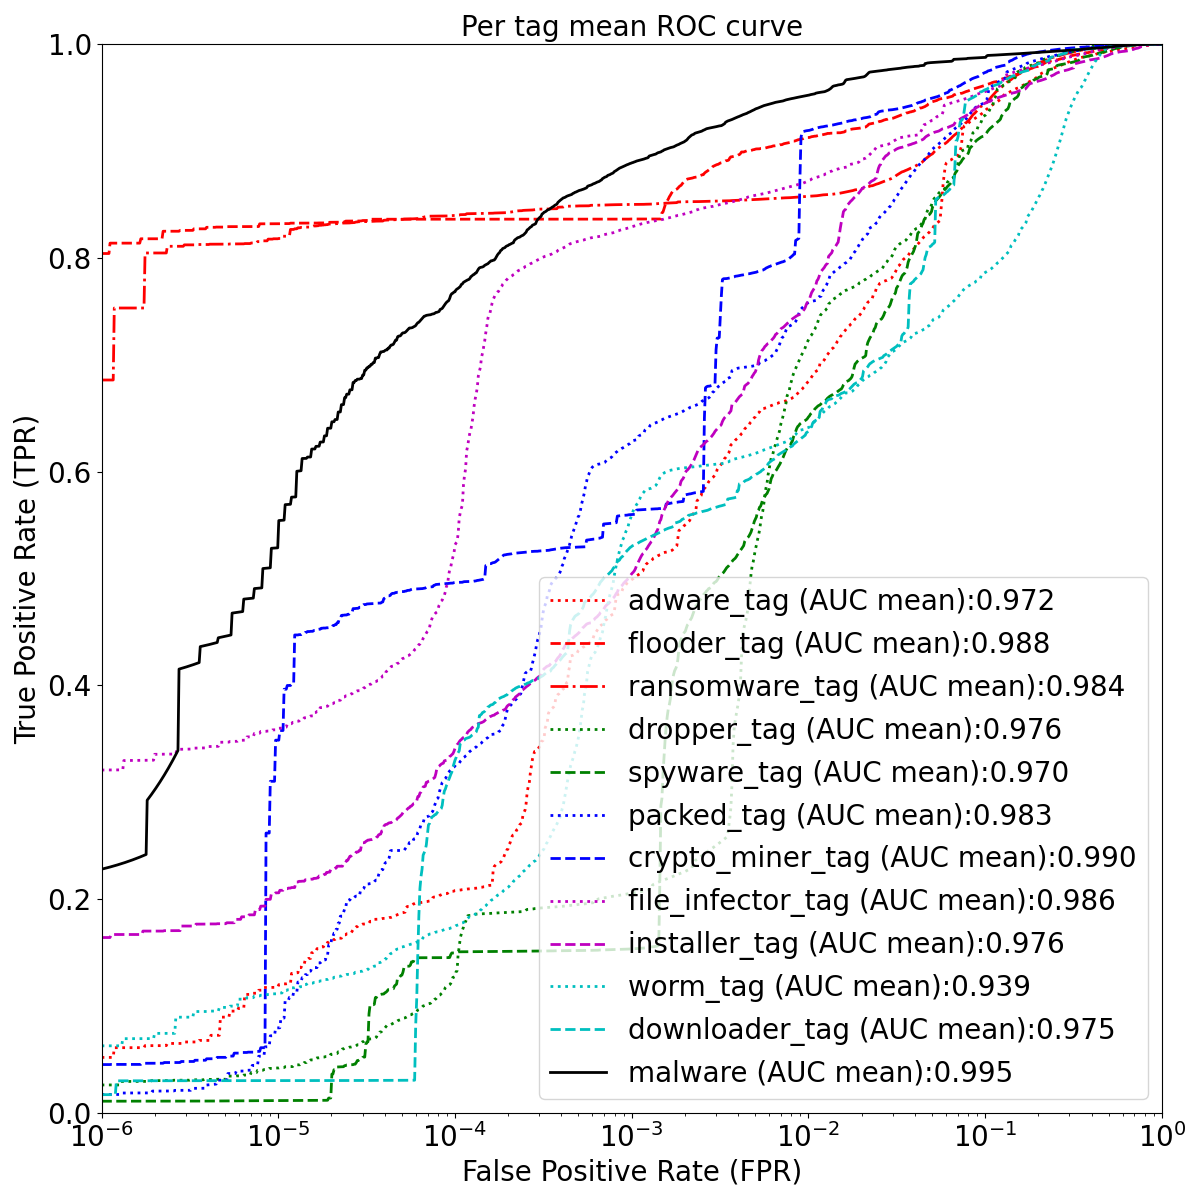
\includegraphics[width=0.6\textwidth]{./results/all_mean_roc_proposedModel.png}
        \vspace*{-0.2cm}
        \caption[Tags prediction task Proposed Model mean ROC curve]{Mean ROC curve and AUC statistics of \textBF{Proposed Model} for the tags/labels. The line represents the \textit{mean} TPR at a given FPR. Statistics were computed over \textBF{3} training runs, each with random parameter initialization.}
        \label{fig:allMeanRocProposedModel}
    \end{figure}
}